\documentclass{beamer}
\usetheme{Madrid}
\colorlet{beamer@blendedblue}{green!40!black}
\setbeamertemplate{bibliography item}{\insertbiblabel}
\setbeamertemplate{caption}[numbered]
\makeatletter
\setbeamertemplate{footline}{%
    \leavevmode%
    \hbox{%
    \begin{beamercolorbox}[wd=.25\paperwidth,ht=2.25ex,dp=1ex,center]{title in head/foot}%
      \usebeamerfont{title in head/foot}\insertshorttitle
    \end{beamercolorbox}%
    \begin{beamercolorbox}[wd=.5\paperwidth,ht=2.25ex,dp=1ex,center]{author in head/foot}%
        \usebeamerfont{author in head/foot}\insertshortauthor\expandafter\beamer@ifempty\expandafter{\beamer@shortinstitute}{}{~~(\insertshortinstitute)}
    \end{beamercolorbox}%
        \begin{beamercolorbox}[wd=.25\paperwidth,ht=2.25ex,dp=1ex,right]{date in head/foot}%
            \usebeamerfont{date in head/foot}\insertshortdate{}\hspace*{2em}
            \insertframenumber{} / \inserttotalframenumber\hspace*{2ex} 
        \end{beamercolorbox}}%
        \vskip0pt%
    }
\makeatother
\usepackage{xcolor}
\usepackage{amsmath, amssymb, amsthm}
\usepackage{physics}
\usepackage{float, subcaption, graphicx} \usepackage{hyperref}

\title[Stability of Transonic Flow]{Stability of the Transonic Plasma Flow in the Magnetic Nozzle}
\author[HF(hunt.feng@usask.ca), SA(andrei.smolyakov@usask.ca)]
{
  Hunt Feng\\ 
  Supervisor: Andrei Smolyakov
}
\institute[]
{
  Faculty of Physics and Engineering Physics \\  
  University of Saskatchewan
}
\date{}
\titlegraphic{
   
\includegraphics[width=0.3\linewidth]{figures/usask_usask_colour.png}
}

\begin{document}
\frame{\titlepage}

\chapter{Introduction}
\section{Motivation}
With the depletion of the earth's resources, the development of space has become a topic that cannot be avoided for mankind. To make space development possible, the necessary space propulsion technology must progress. 

To understand the advantage of electric propulsion. We need to review how propulsion system works. In order to change momentum, a spacecraft needs to expel parts of its mass, the propellant. The motion can be fully characterized by the Newton's second law.
\[ \dv{(mv_e)}{t} = \dot{m}v_e \]
where $m$ is the propellant mass, and $v_e$ is the exhaust velocity.

In 1903, a Russian and soviet rocket scientist, Konstantin Tsiolkovsky, derived the famous rocket equation that relates the change of a rocket's velocity to its exhaust velocity, and the mass of the rocket and propellant,
\[ \Delta v = -v_e \ln(\frac{M}{M+m}) \]
where $\delta v$ is the change in velocity of the spacecraft, $M$ is the mass of spacecraft without propellant, and $m$ is the mass of propellant.

From the Tsiolkovsky rocket equation, we see that higher the ratio between empty rocket and fueled rocket, higher the final velocity. Moreover, if the mass ratio is fixed, then a high exhaust velocity is needed in order to achieve higher final speed. In a chemical rocket, the exhaust velocity of propellant is limited by the temperature of the combustion fuels.

\begin{figure}[H]
	\centering
	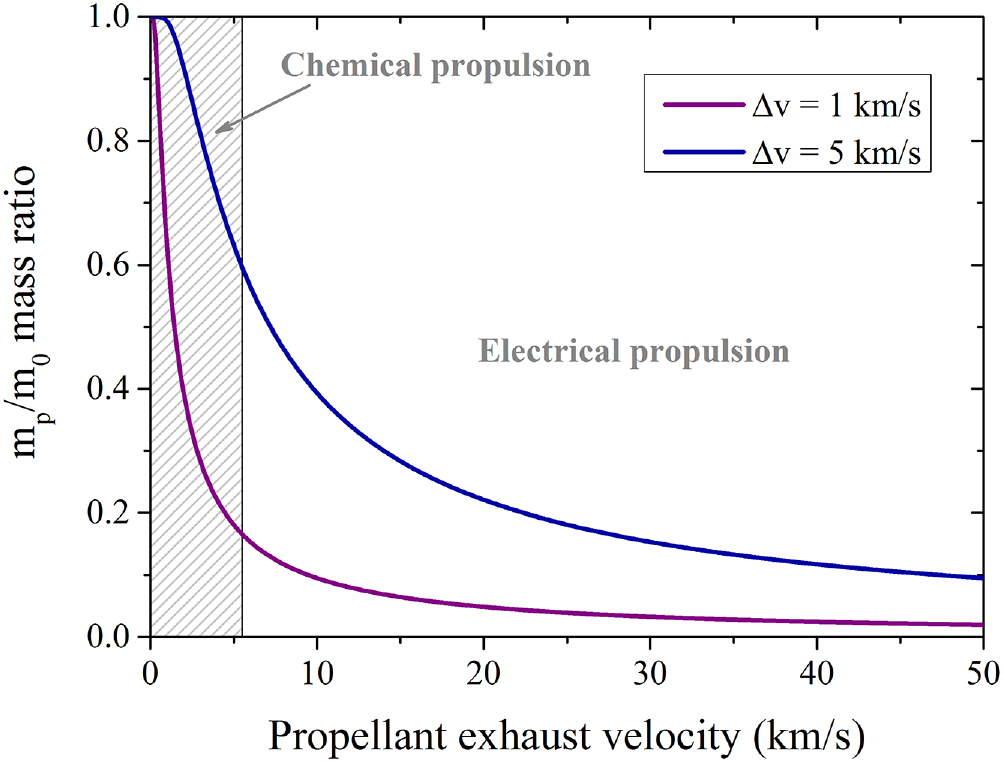
\includegraphics[width=0.7\linewidth]{img/introduction/mass_ratio_vs_exhaust_velocity}
	\caption{Ratio of the propellant mass to the initial mass as a function of the exhaust velocity ve for two values of the velocity increment $\Delta v$ . The dashed area corresponds to the domain of chemical propulsion with ve below 5.5 $km \, s^{-1}$. \cite{mazouffre_electric_2016} }
	\label{fig:massratiovsexhaustvelocity}
\end{figure}



\section{Magnetic Nozzle}
Magnetic nozzle is a convergent-divergent magnetic field that guides, expands and accelerates a plasma jet into vacuum for the purpose of space propulsion. \cite{andersen_continuous_1969,boswell_experimental_2004,williams_fusion_2003} The configuration is of the magnetic field in the magnetic nozzle plays a similar role to the walls of a Laval nozzle, see Fig. \ref{fig:magnetic-nozzle}. The plasma flow starts from subsonic at one end can be accelerated to supersonic at the other end. 

One advantage of magnetic nozzle is that it can operate contactlessly. Since the magnetic nozzle converts the plasma thermal energy into kinetic energy, so the thrust and specific impulse are strongly dependent on the temperature of the plasma flow. Higher the plasma temperature, more effective the plasma thruster. The magnetic field in the magnetic nozzle bounds the hot plasma, and therefore prevents the contact of the nozzle wall and the hot plasma jet. Hence, magnetic nozzle is an appealing plasma acceleration technology. Fig. \ref{fig:massratiovsexhaustvelocity} shows the comparison between magnetic nozzle and traditional chemical rocket.

Moreover, the configuration of magnetic field in magnetic nozzle is important for many other applications,\cite{smolyakov_quasineutral_2021} such as the magnetic divertors in fusion devices,\cite{ryutov_divertor_2016,togo_characteristics_2019} and is also related to the solar wind and accretion flow.\cite{jockers_stability_1968,aikawa_stability_1979} 

\begin{figure}[H]
	\centering
	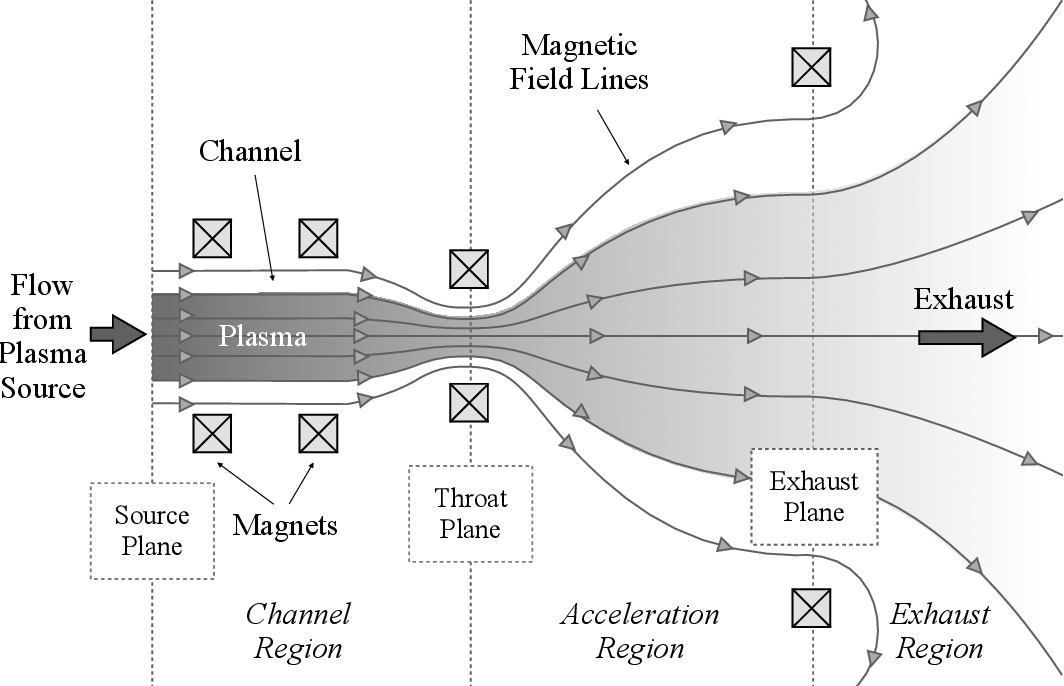
\includegraphics[width=0.7\linewidth]{img/introduction/magnetic_nozzle}
	\caption{Example of a magnetic nozzle configuration. In our models, we define the magnetic nozzle as the region downstream from the throat plane, which can be further divided into an acceleration region and exhaust region. The channel connects the plasma source (not shown) with the magnetic nozzle. \cite{little_performance_2015}}
	\label{fig:magnetic-nozzle}
\end{figure}


\section{Plasma Instability}
However, the plasma motion is determined by the Lorentz force, the nature of the nonlinearity of the motion makes it hard to predict analytically. Since the construction of Tokamak, people underestimated the difficulty of describing plasma motion. Hence, in order to maintain the equilibrium in the Tokamak, people start analyzing the stability of plasma. Nowadays, the study of plasma instabilities is an important area in plasma physics. 

Consider a plasma system in at equilibrium, we introduce a small perturbation to it. The stability of the system determines if the perturbations will grow, oscillate, or be damped out. Similar to the study of mechanical stability at equilibrium. See Fig. \ref{fig:stability-visualization}.

\begin{figure}[H]
	\centering
	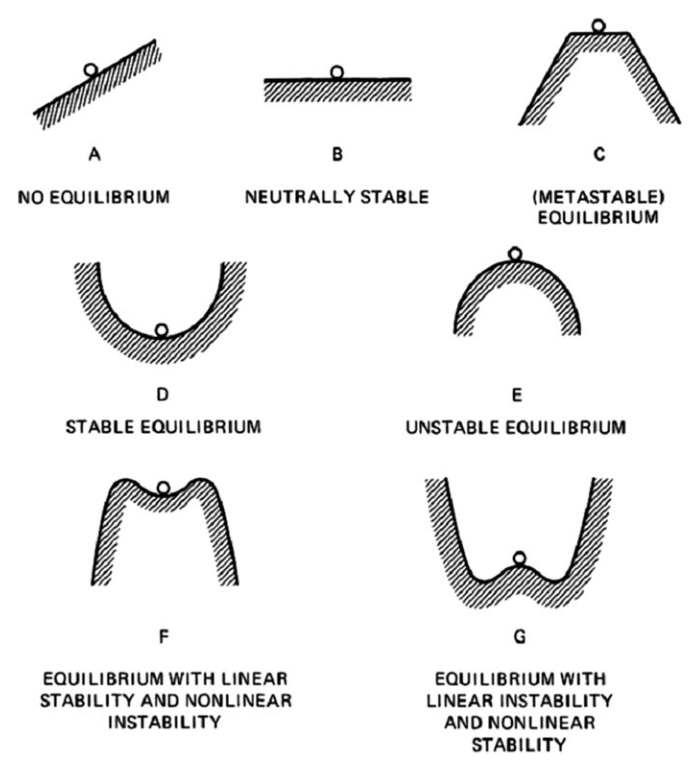
\includegraphics[width=0.7\linewidth]{img/introduction/stability_visualization}
	\caption{Mechanical analogy of various types of equilibrium. \cite{chen_introduction_2016}}
	\label{fig:stability-visualization}
\end{figure}


\subsection{Illustration: Two-Stream Instability}
We take the famous two-stream instability as an illustration. Let the plasma be cold ($k_BT_e = k_BT_i = 0$), let there be no magnetic field ($B_0=0$). The linearized continuity equations are
\begin{align} 
	\pdv{n_{i1}}{t} + n_0\pdv{v_{i1}}{x} &= 0  \label{eq:two-stream-continuity1} \\
	\pdv{n_{e1}}{t} + n_0\pdv{v_{e1}}{x} + v0\pdv{n_{e1}}{x} &= 0 \label{eq:two-stream-continuity2}
\end{align}

And the linearized equations of motion are
\begin{align} 
	Mn_0\pdv{v_{i1}}{t} &= en_0E_1  \label{eq:two-stream-eom1} \\
	mn_0\left(\pdv{v_{e1}}{t} + v_0\pdv{v_{e1}}{x}\right) &= -en_0E_1 \label{eq:two-stream-eom2}
\end{align}
Here $v_0$ is the velocity of electron respect to the ions (the ion velocity at equilibrium is taken to be $v_{i0}=0$), $n_0$ is the equilibrium density of both ion and electron, $v_{i1}$ and $v_{e1}$ are perturbed velocity of ions and electrons, and $E_1$ is the perturbed electron field.

If we assume perturbed electric field takes the wave form
\[ E_1 = E\exp(i(kx-\omega t)) \]
Plug this perturbed electric field into Eq.(\ref{eq:two-stream-eom1}) and (\ref{eq:two-stream-eom2}), then we can solve for $v_{i1}$ and $v_{e1}$,
\begin{align*}
	v_{i1} &= \frac{ie}{M\omega} E \\
	v_{e1} &= -\frac{ie}{m}\frac{E}{\omega-kv_0}
\end{align*}

Using the perturbed velocities, the continuity equations Eq.(\ref{eq:two-stream-continuity1}) and (\ref{eq:two-stream-continuity2}) yields
\begin{align*}
	n_{i1} &= \frac{ien_0k}{M\omega^2} E \\
	n_{e1} &= \frac{iekn_0}{m(\omega-kv_0)^2}E
\end{align*}

Finally, plug them into the Poisson's equation
\[ \epsilon_0 \pdv{E_1}{x} = e(n_{i1}-n_{e1}) \]
We now have the dispersion relation
\[ 1 = \omega_p \left[\frac{m/M}{\omega^2}+\frac{1}{(\omega-kv_0)^2}\right] \]

Solving this equation for $\omega$, there is chance we will get complex frequency,
\[ \omega = \omega_r + i\omega_i \]
where $\omega_r, \omega_i \in\mathbb{R}$. Then the perturbed electric field becomes
\[ E_1 = E\exp(i(kx-\omega_rt))\exp(\omega_it) \]

When $\omega_i < 0$, it is a damped wave, when $\omega_i > 0$, it grows exponentially and therefore unstable. Since the complex root comes with pair, as long as $\omega_i\neq 0$, one of the roots must correspond to an unstable wave. The following graph shows the two-stream instability in phase space.

\begin{figure}[H]
	\centering
	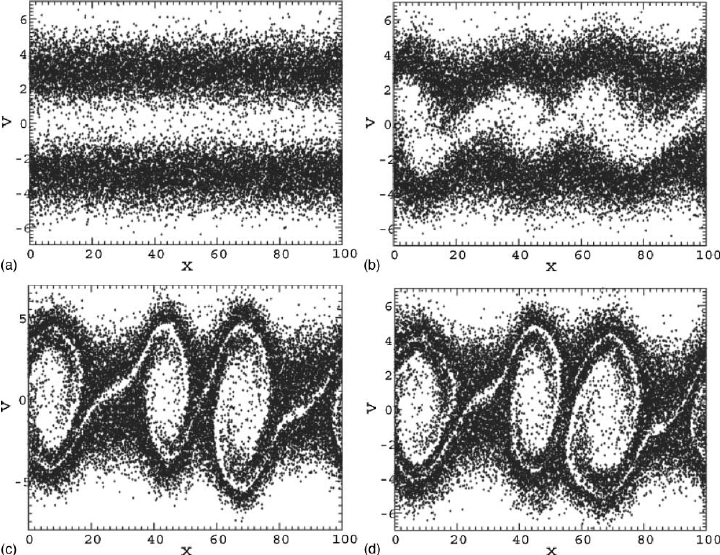
\includegraphics[width=0.7\linewidth]{img/introduction/two_stream_instability}
	\caption{Visualization of two-stream instability in the phase space. (a) Initially the ion and electron flow are in opposite direction. (b) The velocity of both flows start to oscillate. (c) Chaotic behavior occurs. (d) The chaotic behavior continues. \cite{ha_nonlinear_2011}}
	\label{fig:two_stream_instability}
\end{figure}

\subsection{Stability of Configurations Similar to Magnetic Nozzle}
Accretion flow has configuration similar to the magnetic nozzle. It is natural to find studies of stability the accretion flow. However, the results are still debatable. \cite{keto_stability_2020,aikawa_stability_1979,stellingwerf_stability_1978}


\section{Goals of this Thesis}
The goals of this thesis is to first study the spectral method for solving the instability problem. When using the spectral method, it is necessary to understand different discretizations of the operators, such as finite difference, finite element and DVR method.

Once the spectral method is introduced, we can use it to study the instability of plasma in magnetic nozzle. We can use different discretization techniques, and compare the results from different methods.

Finally, we need to take care of the filtering of the spectral pollution.


\section{Thesis Outline}
The theory of spectral methods will be discussed in chapter \ref{chap:spectral_method}. In this chapter, different discretiation methods will be introduced. Moreover, a very important concept, spectral pollution, will be introduced in detailed in the final section of this chapter.

Then, in chapter \ref{chap:governing_equations} is the discussion of governing equations and its linearization. The formulation of the problem will be derived in this chapter.

In chapter ??, we ill use the equations derived in chapter \ref{chap:governing_equations} to conduct numerical experiments. The goal is to investigate the frequency of each modes. The filtering methods of spurious modes will be introduced.

Conclusion will in chapter ??


\chapter{Singular Perturbation} \label{chap:singular-perturbation}
This chapter is dedicated to analyze the polynomial eigenvalue problem with transonic velocity profiles. We will first show the existence of the singularity of Eq.(\ref{eq:polynomial-eigenvalue-problem}), then we will discuss the concept of singular perturbation and the way we solve the problem.

\section{Presence of Singularity in Transonic cases} \label{sec:presence-of-singularity}
In order to see the existence of the singularity, we rearrange the terms the polynomial eigenvalue problem, Eq.(\ref{eq:polynomial-eigenvalue-problem}),
\begin{equation} \label{eq:singular-perturbation-problem}
	\begin{aligned}
		  & (1-v_0^2)\pdv[2]{\tilde{v}}{z}                                                                                                                             \\
		+ & \left(2i\omega v_0 - \left(3v_0 + \frac{1}{v_0}\right)\pdv{v_0}{z}\right)\pdv{\tilde{v}}{z}                                                                \\
		+ & \left[2i\omega\pdv{v_0}{z} -\left(1 - \frac{1}{v_0^2}\right)\left(\pdv{v_0}{z}\right)^2 - \left(v_0 + \frac{1}{v_0}\right)\pdv[2]{v_0}{z} \right]\tilde{v} \\
		= & 0
	\end{aligned}
\end{equation}
This is a second order ordinary differential equation defined on region $[-1,1]$.

For transonic (accelerating and decelerating) velocity profiles (Fig.\ref{fig:velocity-profiles}), the plasma flow is at sonic point at the throat of the nozzle, $v_0(0)=1$. Therefore, the highest order term vanishes at $z=0$. This causes the failure of spectral method, see Fig.(\ref{chap:discussion}). It can be proved that $z=0$ is a regular singular point.

\begin{figure} [htbp]
	\centering
	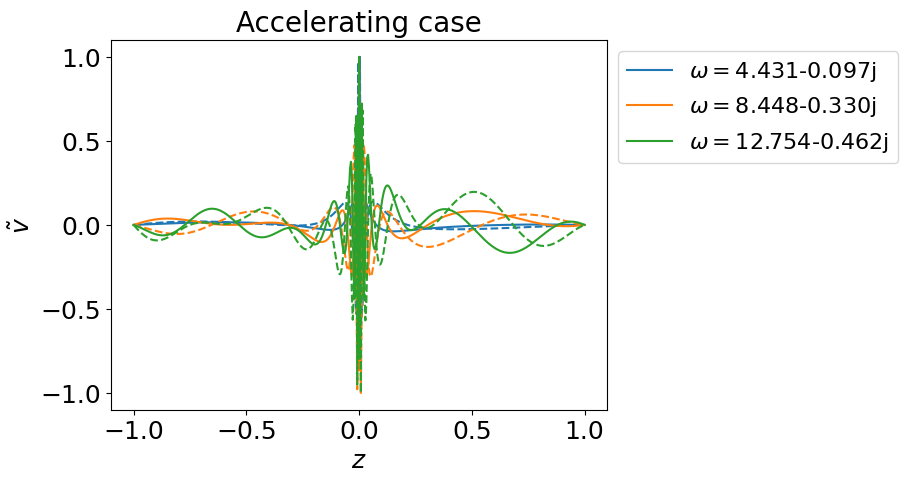
\includegraphics[width=0.7\textwidth]{img/results-bad-accelerating-v}
	\caption{An attempt to solve the polynomial eigenvalue problem, Eq.(\ref{eq:polynomial-eigenvalue-problem}) using finite-difference. Eigenfunctions are squeezed to the center of the nozzle due to the existence of the singularity at $z=0$.}
	\label{fig:failure-of-spectral-method}
\end{figure}

\section{Connection of Singularity to Black Hole}
\subsection{Acoustic Analog to Tortoise Coordinate}

\section{Singular Perturbation Problem}
Consider Eq.(\ref{eq:polynomial-eigenvalue-problem}) as a boundary value problem by fixing the value of $\omega$,
The boundary value problem Eq.(\ref{eq:singular-perturbation-problem}) is defined on region $[-1,1]$, but the boundary values are defined on $z=-1$ and $z=0$. This is because to extract a regular solution near the singularity, we need to assume the solution is finite at the throat of the nozzle, $z=0$. This condition serves as a boundary value to the problem. Together with the boundary condition at the entrance of the nozzle, $\tilde{v}(-1) = 0$, the solutions to the boundary value problem, Eq.(\ref{eq:singular-perturbation-problem}) is fully determined up to a set of eigenvalues.

As we discuss in the earlier section, Sec.\ref{sec:presence-of-singularity}, $(1-v_0^2)$ is 0 at the nozzle throat $z=0$ since $v_0(z)$ is now a transonic velocity profile. This makes the problem a first order ordinary differential equation,
\[
	\left( 2i\omega - 4\eval{\pdv{v_0}{z}}_{z=0} \right)\pdv{\tilde{v}}{z}
	+ \left[2i\omega\eval{\pdv{v_0}{z}}_{z=0} - 2\eval{\pdv[2]{v_0}{z}}_{z=0} \right]\tilde{v}  = 0
\]
It is clear that the solution to this first order ODE has a totally different characteristics than the solution in the neighborhood of $z=0$. That means we cannot simply set $(1-v_0^2)$ to 0 and get an asymptotic approximation to the solution of Eq.(\ref{eq:singular-perturbation-problem}) near $z=0$. This is exactly the characteristics of singular perturbation problem.

\section{Expansion at Singularity}
The singularity is a regular singular point, we are able to extract finite solution near the singularity. In order to do so, we need to expand terms in Eq.(\ref{eq:singular-perturbation-problem}) about the singularity.

The first task is to linearize the terms with $v_0$ about the singularity. The linearization of $v_0(z) = 1 + v_0'(0)z$ is a good approximation to the original function $v_0(z)$ because the transonic velocity profiles are straight in the neighborhood of $z=0$, as we can see from Fig.\ref{fig:velocity-profiles}. Therefore, through some simple algebra we obtain,
\begin{equation}
	\begin{aligned}
		1-v_0^2              & = -2v_0'(0)z    \\
		3v_0 + \frac{1}{v_0} & = 4 + 2v_0'(0)z \\
		1-\frac{1}{v_0^2}    & = 2v_0'(0)z     \\
		v_0 + \frac{1}{v_0}  & = 2
	\end{aligned}
\end{equation}

Then Eq.(\ref{eq:singular-perturbation-problem}) becomes
\begin{equation} \label{eq:perturbed-equation-full}
	\begin{aligned}
		- & 2v_0'(0)z\pdv[2]{\tilde{v}}{z}                                              \\
		+ & [2i\omega - 4v_0'(0) + (2i\omega - 2v_0'(0))z]\pdv{\tilde{v}}{z}            \\
		+ & \left[\omega^2 + 2i\omega v_0'(0) - 2v_0''(0) - 2v_0'(0)^3z\right]\tilde{v}
		= 0
	\end{aligned}
\end{equation}

In fact, we can further simply the equation by dropping all $z$ terms except the first term (second-order derivative term). It can be shown that dropping the $z$ terms in Eq.(\ref{eq:perturbed-equation-full}) does not affect the first order correction ($\tilde{v}$ is the same up to $z$ term), it is an acceptable approximation.

\[ - 2v_0'(0)z\pdv[2]{\tilde{v}}{z}
	+ (2i\omega - 4v_0'(0))\pdv{\tilde{v}}{z}
	+ (\omega^2 + 2i\omega v_0'(0) - 2v_0''(0))\tilde{v}
	= 0 \]

Dividing by the first coefficient, we have
\begin{equation}
	z\pdv[2]{\tilde{v}}{z} + a\pdv{\tilde{v}}{z} + b\tilde{v} = 0
	\label{eq:perturbed-equation}
\end{equation}
where
\[ a = \frac{2i\omega - 4v_0'(0)}{-2v_0'(0)}; \quad
	b = \frac{\omega^2 + 2i\omega v_0'(0) - 2v_0''(0)}{-2v_0'(0)}
\]

Use Frobenius method, we assume the velocity perturbation can be written as a power series in $z$,  $\tilde{v} = \sum_{n\geq 0}c_nz^{n+r}$. By substituting the power series into Eq.(\ref{eq:perturbed-equation}) we have
\[ \sum_{n \geq 0} (n+r)(n+r+1) c_n z^{n+r-1} + a(n+r)c_nz^{n+r-1} + bc_nz^{n+r} = 0\]
Shift the power of the last term we get
\[ \sum_{n \geq 0} (n+r)(n+r+1) c_n z^{n+r-1} + a(n+r)c_nz^{n+r-1} + \sum_{n \geq 1} bc_{n-1}z^{n+r-1} = 0\]

Setting $n=0$, we get the indicial equation
\[ c_0 r(r-1) + c_0 ar = 0 \Rightarrow c_0r(r+a-1) = 0 \]
We get two different roots, $r=0$ and $r=1-a$. They correspond to finite solution and diverging solution near the singularity, respectively.

The coefficients are given by recurrence relation
\[ (n+r)(n+r-1)c_n + a(n+r)c_n + bc_{n-1} = 0
	\Rightarrow
	c_n = \frac{-bc_{n-1}}{(n+r)(n+r-1+a)}
\]
Solving this relation we get explicit expression for $c_n$, $n\in\mathbb{N}$,
\begin{equation}
	\begin{aligned}
		c_n & = \frac{(-1)^n b^n c_0}{\prod_{k=0}^{n-1} (n+r-k)(n+r-1+a-k)}              \\
		    & = (-1)^n b^n c_0 \frac{\Gamma(r+1)\Gamma(r+a)}{\Gamma(n+r+1)\Gamma(n+r+a)}
	\end{aligned}
	\label{eq:coefficient}
\end{equation}

Therefore, we successfully extracted the regular solution (corresponding to the root $r=0$) in the form of power series,
\begin{equation} \label{eq:regular-solution}
	\begin{aligned}
		\tilde{v} & = c_0 + c_1z + c_2z^2 + \cdots                               \\
		          & = c_0 - c_0\frac{b}{a}z + c_0\frac{b^2}{2a(1+a)}z^2 + \cdots
	\end{aligned}
\end{equation}

It is worth to mention that the diverging solution (corresponding to the root $r=a$) goes like
\[ \tilde{v}(z) \sim z^{1-a} = z^{-1-\omega_i/v_0'(0)}z^{i\omega_r/v_0'(0)}  \]
where $\omega = \omega_r + i\omega_i$. Meaning that the solution will be divergent if and only if $\omega_i > -v'(0)$.

\section{Shooting Method}
Shooting method can be used to solve eigenvalue problem with specified boundary values,
\begin{equation} \label{eq:boundary-eigenvalue-problem}
	g(\tilde{v}(z);\omega) = 0,
	\quad
	z_l \leq z \leq z_r,
	\quad
	\tilde{v}(z_l) = \tilde{v}_l, \tilde{v}(z_r) = \tilde{v}_r
\end{equation}
where $\omega$ is the eigenvalue to be solved.

Suppose an eigenvalue problem can be formulated as
\[ \dv{z}\mathbf{u} = \mathbf{f}(\mathbf{u},z;\omega),
	\quad
	z_l<z<z_r,
	\quad
	\mathbf{u}(z_l) = \mathbf{u}_l
\]
where $\mathbf{u}\in\mathbb{R}^2$. Fixed an $\omega$, we can approximate $\mathbf{u}(z_r)$ by applying algorithms such as Runge-Kutta or Leap-frog.

Define $F$ by $F(\mathbf{u}_l;\omega)=\tilde{v}(z_r;\omega)$. This function $F$ takes in the initial value $\mathbf{u}_l$ and a fixed $\omega$, and outputs the "landing point" $\tilde{v}(z_r;\omega)$. If $\omega$ is an eigenvalue of Eq.(\ref{eq:boundary-eigenvalue-problem}), then $\tilde{v}(z_r;\omega) = \tilde{v}_r$. Now we can find eigenvalues to Eq.(\ref{eq:boundary-eigenvalue-problem}) by solving the roots to the scalar equation
\[h(\omega) = F(\mathbf{u}_l;\omega) - \tilde{v}_r\]

Having this higher view of shooting method in mind, we first transform Eq.(\ref{eq:polynomial-eigenvalue-problem}) to a IVP,
\begin{align*}
	v' & = u                        \\
	u' & = \frac{-1}{1-v_0^2}\left[
		\omega^2v + 2i\omega(v_0+v_0'v) - \left(3v_0 - \frac{1}{v_0}\right)v_0'u - \left(1-\frac{1}{v_0}^2\right)(v_0')^2v - \left(v_0+\frac{1}{v_0}v_0'' v\right)
		\right]
\end{align*}
and $v(0)=c_0=1,u(0)=c_1=(2i\omega v_0'-2v_0'')/2v_0'$. Moreover, $u'(0)=c_2=-((v_0')^4+(2i\omega v_0' + (v_0')^2 - v_0'')(i\omega v_0' - v_0''))/(v_0'(2i\omega-6v_0'))$.

In order to get initially value for cases with transonic velocity profiles, we need to expand the solution at the singularity.



\newpage
\begin{frame}[allowframebreaks] {References}
  \tiny
  \nocite{*}
  \bibliographystyle{abbrv}
  \bibliography{references}
\end{frame}

\end{document}
